%
%% Please do not remove author note!
%%%
%%%% Created by Kacper B Sokol (k.sokol.2011 [at] my.bristol.ac.uk)
%%%
%% Please do not remove author note!
%

\documentclass[11pt, letterpaper]{article}            % report | leqno, pdflatex

% \usepackage[]{algorithm2e}
% \usepackage[usenames,dvipsnames]{color}
% \usepackage[letterspace=3pt]{microtype} % linespacing

\usepackage[left=3.17cm, right=3.17cm, bottom=2.54cm, top=2.54cm]{geometry}
\usepackage{graphicx}                                                 % graphics
\usepackage{color}                                              % custom colours
\usepackage{lipsum}                                        % just a space filler
\usepackage{soul}												% letter spacing
\definecolor{natc}    {RGB}{021,055,090}
\definecolor{subc}    {RGB}{121,121,121}
\definecolor{headc}   {RGB}{034,065,094}
\definecolor{headerc} {RGB}{127,145,173}
\definecolor{footerc} {RGB}{128,128,128}
\definecolor{footerc1}{RGB}{192,192,192}
\definecolor{linec}   {RGB}{237,237,237}
\usepackage[absolute]{textpos}      % absolute positioning of images | showboxes
\usepackage{cite}                                                        % BiTeX
\usepackage[square]{natbib}									  % Harvard citation

\usepackage{datetime}                                              % custom date
\newdateformat{motd}{\monthname[\THEMONTH] \THEYEAR}               % custom date

\usepackage{fontspec}                                      % all different fonts
\usepackage{xcolor}
\usepackage{titlesec}
\defaultfontfeatures{Ligatures=TeX}
\setsansfont{Arial}
\setmainfont{Times New Roman}
\titleformat*{\section}{\fontsize{16}{18}\color{headc}\bfseries\sffamily}
\titleformat*{\subsection}{\fontsize{13}{15}\color{headc}\bfseries\sffamily}
\titleformat*{\subsubsection}{\fontsize{11}{13}\color{headc}\bfseries\sffamily}
\newfontfamily\headerfont[Ligatures=TeX]{Calibri}
\newfontfamily\footerfont[Ligatures=TeX]{Times New Roman}


\usepackage[linktocpage=true]{hyperref}						    % click-able ToC
\usepackage{tocloft}
\renewcommand{\contentsname}							   % ...
	{\fontsize{16}{18}\color{headc}\bfseries\sffamily	   % ...
	Table of Contents}									   % change name for ToC

\setcounter{tocdepth}{3}
\cftsetindents{section}{0.0em}{1.0em}
\cftsetindents{subsection}{1.0em}{2.0em}
\cftsetindents{subsubsection}{2.0em}{3.0em}
% \cftsetindents{paragraph}{0.5in}{0.5in}
% \makeatletter \renewcommand*\l@section{\@dottedtocline{1}{1.5em}{2.3em}} \makeatother
\makeatletter \renewcommand*\l@section{\@dottedtocline{0}{0.0em}{1.5em}} \makeatother
% \renewcommand{\cftsecfont}{\fontsize{19}{13}\color{headc}\bfseries\sffamily}


% define headers and footers
\usepackage{etoolbox,fancyhdr,xcolor}
\pagestyle{fancy}
\newcommand{\footrulecolor}[1]{\patchcmd{\footrule}{\hrule}{\color{#1}\hrule}{}{}} % footer colour
\fancyhead{} % clear all header fields
\renewcommand{\headrulewidth}{0pt} % no line in header area
\fancyhead[LE,LO]{\headerfont\fontsize{9}{11}\selectfont\color{headerc}\textbf{CERN openlab Summer Student Report}}
\fancyhead[RE,RO]{\headerfont\fontsize{9}{11}\selectfont\color{headerc}\textbf{\the\year}}
\fancyfoot{} % clear all footer fields

%%%%%%%%%%%%%%%%%%%%%%%%%%%%%%%%%%%%%%%%%%%%%%%%%%%%%%%%%%%%%%%%%%%%%%%%%%%%%%%%
%%%%%%%%%%%%%%%%%%%%%%%%%%%%%%%%%%%%%%%%%%%%%%%%%%%%%%%%%%%%%%%%%%%%%%%%%%%%%%%%
%%%%%%%%%%%%%%%%%%%%%%%%%%%%%%%%%%%%%%%%%%%%%%%%%%%%%%%%%%%%%%%%%%%%%%%%%%%%%%%%
%%%%%%%%%%%%%%%%%%%%%%%%%%%%%%%%%%%%%%%%%%%%%%%%%%%%%%%%%%%%%%%%%%%%%%%%%%%%%%%%
%%%%%%%%%%%%%%%%%%%%%%%%%%%%%%%%%%%%%%%%%%%%%%%%%%%%%%%%%%%%%%%%%%%%%%%%%%%%%%%%
%%%%%%%%%%%%%%%%%%%%%%%%%%%%%%%%%%%%%%%%%%%%%%%%%%%%%%%%%%%%%%%%%%%%%%%%%%%%%%%%
\usepackage[]{algorithm2e}
\usepackage{amsmath}
\usepackage{amsfonts}    % fancy maths font
\usepackage{mathrsfs}    % fancy maths font
\usepackage{dsfont}      % indocator finction
\usepackage{mathtools}
%%%%%%%%%%%%%%%%%%%%%%%%%%%%%%%%%%%%%%%%%%%%%%%%%%%%%%%%%%%%%%%%%%%%%%%%%%%%%%%%

\begin{document}

\begin{textblock*}{0mm}(-12.2mm,-0.3mm)\noindent \includegraphics*{./gfx/bg.png}\end{textblock*}
\begin{textblock*}{0mm}(144.3mm,238.3mm)\noindent \includegraphics*{./gfx/openlab.png}\end{textblock*}
\begin{textblock*}{150mm}(114.2mm,140.0mm)\noindent
\parbox{8cm}{\bfseries\sffamily\textbf{\fontsize{20}{20}\selectfont\color{natc}Making sense of data streams:}}\\[.3em]
\parbox{8cm}{\bfseries\sffamily\textbf{\fontsize{20}{20}\selectfont\color{natc}Complex Event Processing for Controls Applications}}\\[36pt]
{\bfseries\sffamily\textbf{\fontsize{16}{20}\selectfont\color{natc}\motd\today}}\\[18pt]
{\sffamily\fontsize{14}{20}\selectfont\color{subc}Author:}\\
{\sffamily\fontsize{14}{20}\selectfont\color{subc}Kacper B.\ Sokol}\\[18pt]
{\sffamily\fontsize{14}{20}\selectfont\color{subc}Supervisor(s):}\\
{\sffamily\fontsize{14}{20}\selectfont\color{subc}Filippo Tilaro}\\
{\sffamily\fontsize{14}{20}\selectfont\color{subc}Axel Voitier}\\[18pt]
\textbf{\bfseries\sffamily\fontsize{11}{20}\selectfont\color{subc}CERN openlab Summer Student Report 2014}

\end{textblock*}
~
\thispagestyle{empty}\newpage

\section*{Project Specification}
CERN is currently investigating the usage of data analysis technologies to study the behavior of the industrial control systems. An activity related to these analysis is using Complex Event Processing tools to classify a real abnormal behavior from one generated by a human intervention on the system. This CEP classification will run over textual logs mainly. A list of events to match will be given as input. The selected CEP tools will be either Drools or Esper. The work will consist of installing one of these tools and develop the classification system with it.
\newpage

\section*{Abstract}
This project aims at build a tool to process live stream of data generated by various sensors. The program uses Esper package to receive data feeds, apply user defined rules, and pass resulting information to clustering framework.\\
The last step employs \emph{Affinity Propagation} based clustering algorithm, which choice is motivated by no need of defining number of clusters prior to program initialisation, and documented overall good performance in live analysis cases.\\
Our approach is then compared on against static clustering algorithm, and in-depth results analysis follows.
\newpage

{\fontsize{11}{13}\sffamily\linespread{1.750}\selectfont\tableofcontents}
\thispagestyle{fancy}\newpage

% Start footer here
\fancyfoot{} % clear all footer fields
\renewcommand{\footrulewidth}{0.4pt} % no line in header area
\footrulecolor{linec}
\fancyfoot[LE,LO]{\footerfont\fontsize{9}{11}\selectfont \textcolor{footerc}{\textbf{\thepage~$|$}}~\textcolor{footerc1}{\footerfont\so{\texttt{Page}}}} % \fontfamily{ppl}\selectfont

\section{Introduction}




\subsection{What is CEP?}
\subsection{What is Esper}
\subsection{Why to use it?}
\subsection{Applications}
\subsection{Examples}
\subsubsection{Nuclear plant}
\subsubsection{CEP at CERN}


\section{Model of processing}
\begin{figure}[htbp]
	\centering
	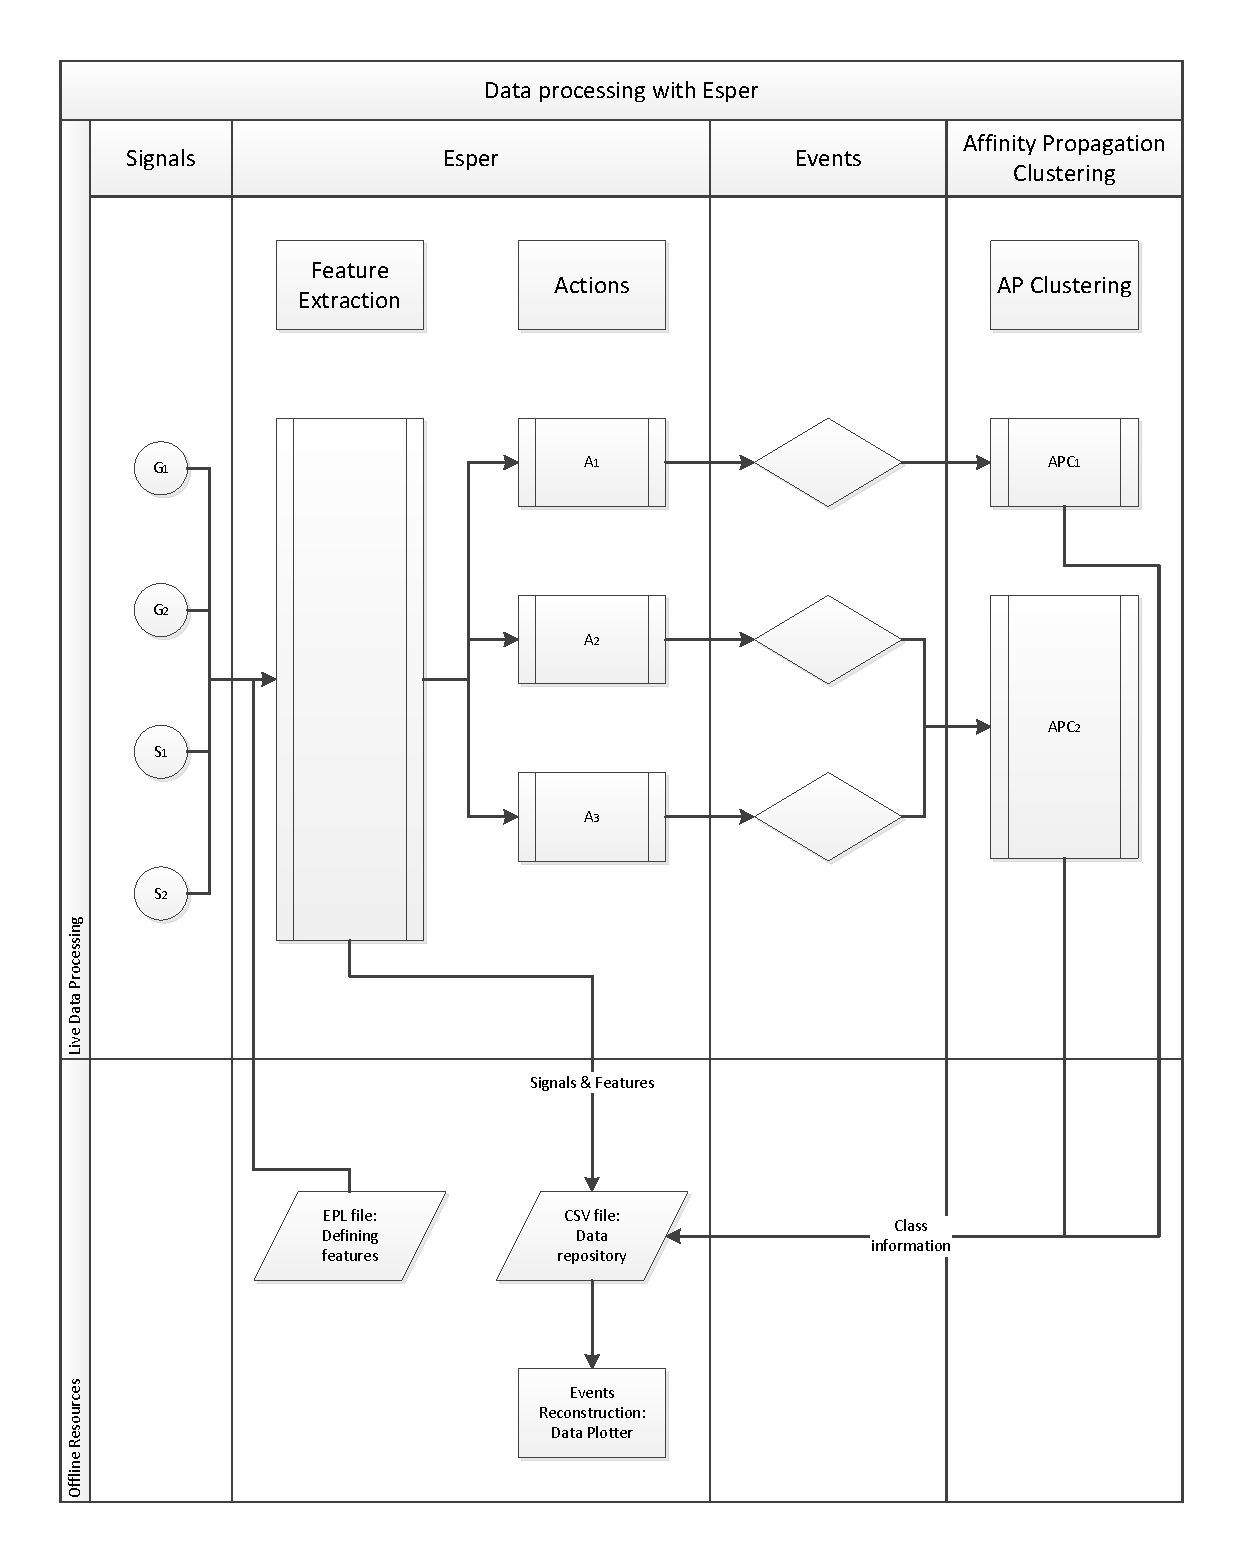
\includegraphics[width=\textwidth]{./gfx/model.pdf}
  \caption{Data processing model.\label{fig:model}}
\end{figure}

\subsection{Esper engine}
\subsection{Generators / signals}
\subsection{Feature extraction}
\subsection{Listeners for change}
\subsection{Clustering with Afinity Propagation}
\begin{figure}[htbp]
	\centering
	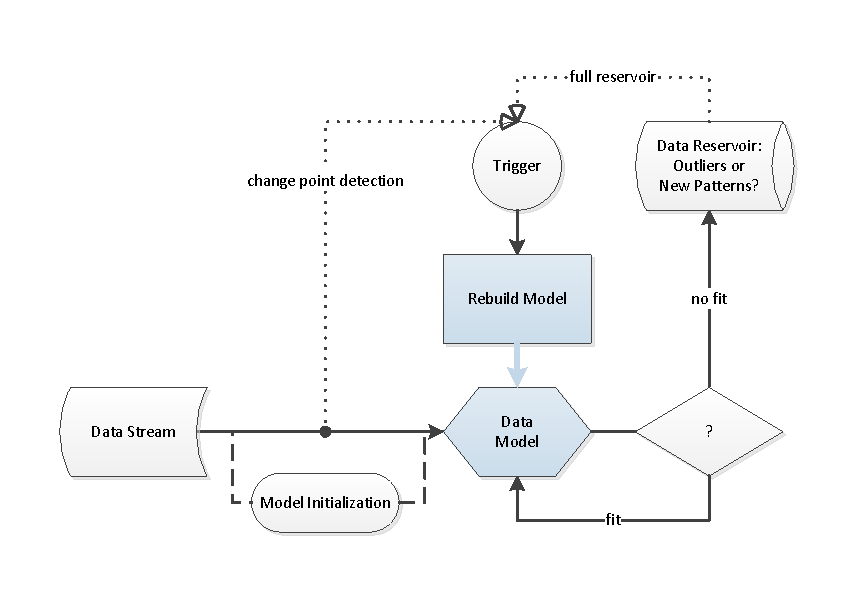
\includegraphics[width=\textwidth]{./gfx/APC.pdf}
  \caption{Stream clustering model.\label{fig:APC}}
\end{figure}

\RestyleAlgo{boxed}
\SetAlCapSkip{1em}
\LinesNumbered
\vspace{2cm}
\begin{algorithm}[h]
  \KwData{Posterior distributions for each action---$\left\{ 
p_a(\cdot|\mathscr{L}_t,x_t) : a \in \mathscr{A} \right\}$}
  \For{$a \in \mathscr{A}$}{
    \text{sample: }$\mathscr{Q}^\text{Th}_{t,a} \leftarrow 
p_a(\cdot|\mathscr{L}_t,x_t)$ \;
  }
  sample $a_t$ uniformly from $\operatorname{arg\,max}_{a \in \mathscr{A}} 
\mathscr{Q}^\text{Th}_{t,a}$ \;
 \caption{Local Thompson Sampling(LTS).\label{al:LTS}}
\end{algorithm}
\vspace{2cm}

\subsection{Printing / GUI}


\section{Results and comparison}
\subsection{why particulat algorithms were chosen}
\subsection{WEKA algorithms review}

\section{Lookahead}

\section{Conclusions}
Weka classification~\citep{zhang2013data}\\
Do graph colouring in classificationlol~\citep{articleExample}\\

Afinity Propoagation\\

\begin{center} \noindent \line(1,0){250} \end{center}	    % Optional ending line


%% Start References (a.k.a. bibliography)
\newpage								 								 % Optional new page before Bibliography
\bibliography{bibliography.bib}{}
\bibliographystyle{plainnat}

\end{document}
